\chapter{Opportunity, Pressure, and the Mirror}

This School of Hard Knocks interview, curated by LazyingArt LLC, begins with public scale and then steadily narrows toward private method. Tom Brady is introduced through titles, rings, and wealth, but the sequence of the conversation does something more interesting than celebrate him: it asks what hidden structure could possibly lie underneath such visible magnitude. No mathematical frame evidence survives from this lecture, so the displayed formulas below are not transcriptions from a board. They are cautious companion notation drawn from the transcript itself, meant to clarify the order of Brady's claims without overwhelming them.

\section{Scale, Chicago, and the First Reduction}

The host stages the meeting in Chicago, at one of Brady's recent businesses, and he begins in the language of spectacle: greatest of all time, seven Super Bowls, three MVPs, hundreds of millions of dollars. We should keep that opening scale, because the first teaching move of the interview depends on it. The interview must first enlarge Brady in order to make his first reduction feel sharp.

Asked how he made his millions, Brady does not begin with brand arithmetic, post-career ownership, or fame as such. He begins with football labor: hard work on the field, taking hits, releasing the ball quickly, and throwing to teammates. That answer is already a kind of discipline. The visible money is pushed downstream of an invisible operating process.

The next move is even more important. When the host calls him the greatest, Brady declines the comparison and says, instead, that he tried to do the best he could with the opportunities he got. That is the first real principle of the chapter. We can write it as a distinction:
\begin{equation}
O_{\text{given}} \neq O_{\text{others}}.
\end{equation}
Here \(O_{\text{given}}\) denotes the opportunities actually available to the agent, while \(O_{\text{others}}\) denotes the opportunities visibly allocated elsewhere. Brady's point is not that these two sets are equal, or should be equal, but that a life can be destroyed by confusing them.

A companion formulation is then
\begin{equation}
\max \operatorname{Use}(O_{\text{given}})
\qquad \text{while refusing to index one's standard to} \qquad
O_{\text{others}}.
\end{equation}
The notation is editorial, but the logic is already in the transcript. Brady's early answer does not optimize rank. It optimizes use.

\subsection{Question \& Answer}

\paragraph{Question.} What exactly are we meant to optimize when the world appears to be giving other people more?

\paragraph{Answer.} The interview's first answer is that our work should be indexed to what is actually in hand. This does not deny asymmetry. It refuses to let asymmetry become the organizing variable of action. Brady's standard is not comparison but conversion: use the rep, the chance, the role, the day that is actually yours.

\section{Nine Years of Hidden Formation}

Once the interview has replaced glamour with opportunity, it moves backward in time. Brady says that through high school and college he had to work very hard simply to become a starter, and later to become a contributor. This is the transcript's first serious timescale. Greatness is being relocated from the moment of fame to the long prehistory in which no one much was watching.

He compresses those years into a rough horizon:
\begin{equation}
T_{\text{apprenticeship}} \approx 9\ \text{years}.
\end{equation}
We should take this as Brady's own pedagogical timescale, not as a demographic theorem. The point is that the formation interval is long, and it is long before the public notices.

The lecture then makes a subtle move. Brady says that by the time he reached the professional level, he already had self-confidence because he had overcome so much when no one was paying attention. In other words, confidence appears late, but it is manufactured early. A cautious update rule is useful here:
\begin{equation}
B_{t+1}=B_t+\Delta B_t,
\qquad
\Delta B_t>0
\ \text{when adversity is survived rather than avoided.}
\end{equation}
Here \(B_t\) is merely a companion variable for self-belief. The interview is not offering a psychological measurement. It is saying that belief was accumulated from lived difficulty.

The same logic is sharpened by institutional doubt. Asked who doubted him, Brady answers with a memorable piece of league arithmetic:
\begin{equation}
N_{\text{teams}}=32,
\qquad
R_{\text{passed}}=6.
\end{equation}
Whether or not we formalize the draft any further, the meaning is plain. Public institutions can render a verdict long before the deeper process has finished. That is why the interview repeatedly returns to the person in the mirror. The mirror appears early, not only at the end. It is first the site of self-belief before it becomes the final site of moral judgment.

\subsection{Question \& Answer}

\paragraph{Question.} How is self-belief built when external institutions are not yet confirming it?

\paragraph{Answer.} The transcript's answer is not mystical. Self-belief is not summoned from nowhere. It is built when repeated obscurity, disappointment, and work produce results that the agent has personally survived and therefore personally knows. By the time public success arrives, confidence is no longer a fantasy about the future. It is memory organized into readiness.

\section{Failure, the Comfort Boundary, and Longevity}

The host then presses further: where did the success itself come from? Brady answers with trial and error and with failure. This is a decisive moment in the interview because failure is not treated as an embarrassing detour on the road to mastery. It is treated as one of mastery's causes.

A faithful companion shorthand is
\begin{equation}
\text{failure} \to \text{adaptation} \to \text{confidence}.
\end{equation}
The arrows are not strict logical implication. They mark the direction of formation in the interview's own language. Failure, when metabolized, generates strategic correction; strategic correction repeated often enough generates steadiness.

The comfort-zone language belongs here for the same reason. Brady says we can wake up every day and live within comfort and convenience, repeating the same actions in the same way. Growth demands an exit from that loop. So we may distinguish, schematically,
\begin{equation}
\mathcal{C} \to \mathcal{G},
\end{equation}
where \(\mathcal{C}\) is the comfort regime and \(\mathcal{G}\) the growth regime outside it. The lecture does not define a boundary operator between them, and we should not invent one. It only insists that real expansion occurs by crossing that boundary again and again.

This same part of the interview then flips the question from becoming great to lasting. The host notes that Brady was not the fastest and not the strongest, yet he outlasted everyone. Brady answers with mentors, especially Alex Guerrero, and with discipline around caring for the body. The structure of the argument is worth preserving. The same person who learned to survive failure also learned to preserve performance. Emergence and longevity are not identical problems, but in the interview they are joined by discipline.

\section{Greg Harden and the Reallocation of Attention}

The most exact corrective moment in the lecture is Brady's story about Greg Harden. Brady recounts his own frustration as a sophomore in college, complaining about unequal opportunity. Harden's intervention is memorable because it does not soothe the complaint. It redirects the field of attention altogether. Stop worrying about what you are not getting; attend to what you are getting. If you are given three chances in practice, then use those three chances.

That move can be written as
\begin{equation}
\operatorname{Focus}_t = O_{\text{given},t},
\qquad
\operatorname{Action}_t = \operatorname{Use}(O_{\text{given},t}).
\end{equation}
The example of three practice opportunities matters because it prevents the point from becoming foggy or inspirational in a generic way. The unit of transformation is small. One does not correct a life all at once. One corrects a life by refusing to squander the next actual rep.

The logic may be read in three layers.

\paragraph{Anecdote.} Brady is preoccupied with the opportunities allocated to others.

\paragraph{Claim.} The actionable set is not the opportunity distribution in the abstract, but the opportunities actually available in the local situation.

\paragraph{Mechanism.} Attention is reallocated from resentment to use, and effort becomes legible again.

This is also the point at which accountability enters the conversation in full force. The host compresses the doctrine into a slogan: nobody is coming to save you. Brady answers by widening accountability beyond the isolated self. We are accountable to ourselves first, but also to the people who matter in our life. The important point is that accountability does not erase relationship; it clarifies responsibility inside relationship.

\subsection{Question \& Answer}

\paragraph{Question.} What do we do when opportunity distributions really are unfair?

\paragraph{Answer.} The interview does not ask us to pretend fairness. It asks us to refuse paralysis. We cannot always alter the whole distribution at once, but we can alter whether the opportunities actually present are converted into performance or wasted inside grievance. That is the Harden correction, and Brady presents it as life-changing.

\paragraph{Editorial note.} At this point the source video is interrupted by a long host-run promotion for AI, personal branding, and the School of Mentors community. It belongs to the platform economy of the video rather than to Brady's conceptual sequence. When the interview resumes, the subject has changed. We are no longer on opportunity; we are on pressure.

\section{Pressure as a Rehearsed State}

After the interruption, the conversation re-enters on its strongest technical idea. Brady is asked how he changed his mind to deal with pressure. His answer is not that pressure is conquered by a heroic speech at the last instant. It is that pressure is trained by repeated exposure to states that resemble the real one.

He begins with a direct identification:
\begin{equation}
S_{\text{practice}} \sim S_{\text{game}},
\end{equation}
where \(\sim\) does not mean literal equality. It means deliberate approximation of emotional load, consequence, and decision tempo. Brady says he treated practice like a game. If they scored in practice, he celebrated as though it were game day. He wanted the emotions of the game to become familiar before the official game arrived.

The interview then adds a more concrete layer. In the offseason, throwing with teammates, he would assign decisive semantics to ordinary reps: fourth down, fourth and seven, one shot to win the Super Bowl. Let us record the local rehearsal state as
\begin{equation}
d=4,
\qquad
y=7,
\qquad
\text{task}=\text{score now or lose}.
\end{equation}
The point is not football notation for its own sake. The point is that consequence can be imported into practice before consequence officially exists.

The strongest reconstruction of the mechanism is therefore
\begin{align}
S_{\text{practice}} &\sim S_{\text{game}},\\
\text{simulated stakes} &\to \text{emotional familiarity},\\
\text{emotional familiarity} &\to \text{embodied readiness}.
\end{align}
This is the exact place where the lecture says, in ordinary language, that by February the body already knows and has already been programmed for the experience. We should keep the phrase while remaining careful with it. Brady is describing learned familiarity, not offering a biological theory.

\begin{figure}[h]
\centering
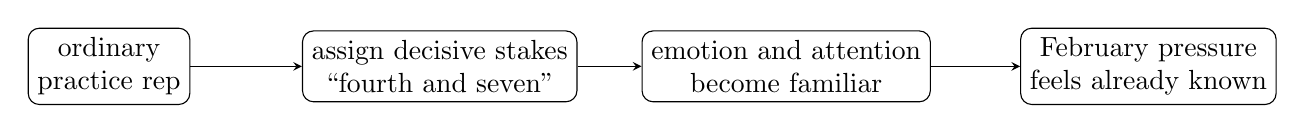
\begin{tikzpicture}[>=stealth]
\node[draw, rounded corners, align=center] (a) at (0,0) {ordinary\\practice rep};
\node[draw, rounded corners, align=center] (b) at (4.2,0) {assign decisive stakes\\``fourth and seven''};
\node[draw, rounded corners, align=center] (c) at (8.6,0) {emotion and attention\\become familiar};
\node[draw, rounded corners, align=center] (d) at (13.2,0) {February pressure\\feels already known};

\draw[->] (a) -- (b);
\draw[->] (b) -- (c);
\draw[->] (c) -- (d);
\end{tikzpicture}
\caption{Transcript-derived schematic of Brady's pressure loop. Practice is not identical to the game, but it can be loaded with enough consequence that the game arrives as a familiar state rather than a wholly alien one.}
\end{figure}

\subsection{Question \& Answer}

\paragraph{Question.} How do we prepare the mind and body for pressure before the real pressure arrives?

\paragraph{Answer.} By refusing to treat pressure as a one-time emergency. We rehearse the state in advance. We attach consequence, emotion, and urgency to ordinary reps until the organism no longer experiences those elements as utterly novel. Then when the true occasion arrives, the stakes are real, but the state is not entirely new.

\section{Super Bowl 51 and Competitive Severity}

The next movement of the interview gives this doctrine an extreme case. The host invokes Super Bowl 51 through the public shorthand \(28\text{-}3\). Brady's own retelling, however, is more sequential. He first remembers the state \(21\text{-}3\), cites Belichick's refusal to concede at that score, and only then recounts the later touchdown that drives the game to \(28\text{-}3\). We should preserve Brady's order rather than overwrite it with the cleaner public legend.

Define the deficit variable by
\begin{equation}
D=\text{opponent score}-\text{own score}.
\end{equation}
Then the two states explicitly narrated in Brady's version of the sequence are
\begin{align}
D_{21\text{-}3} &= 21-3 = 18,\\
D_{28\text{-}3} &= 28-3 = 25.
\end{align}
This is a simple arithmetic example, but it matters because it sharpens the logic of resilience. The situation does not improve first and then invite courage. It worsens first. The doctrine is tested under deterioration.

Belichick's line that 21 points would not be enough functions as a refusal to let the present state exhaust the possible future. Brady's own line that maybe 28 points \emph{is} enough is equally important, because it prevents the chapter from becoming mythological. Doubt remains present. What is prohibited is not doubt, but quitting. In companion notation,
\begin{equation}
D \uparrow \not\Rightarrow \operatorname{Quit}=1.
\end{equation}
More concretely, the interview asks for continued effort at both observed deficit levels:
\begin{equation}
\operatorname{Fight}(D)>0
\qquad
\text{for}
\qquad
D \in \{18,25\}.
\end{equation}
This is still light notation, but it captures the point well. Resilience becomes real only when worsening conditions fail to cancel action.

From here the interview broadens from a single comeback to competition itself. Brady says that anybody can play one game, but that a season is different. The effort gradient across season records is one of the lecture's cleanest ordered claims:
\begin{equation}
E_{4\text{-}13}<E_{9\text{-}8}<E_{12\text{-}5}<E_{15\text{-}2}.
\end{equation}
We should keep this ranking qualitative. It is not a theorem in statistical sports analysis. It is Brady's way of saying that elite outcomes are produced by a steeper daily discipline than mediocre ones. That is why he immediately names the chain underneath the record:
\begin{equation}
\text{habits} \to \text{actions} \to \text{choices} \to \text{season outcome}.
\end{equation}
The record is not the primary object. It is the visible residue of a discipline pipeline.

\section{The Father, the Mirror, and the Lesson of a Life}

The lecture could have ended with competition, but it does not. It turns outward and inward at once, toward fatherhood and the mirror. Brady names his father as his hero. That answer is not sentimental filler. It explains the moral substrate underneath the rest of the chapter: steadiness, integrity, presence, belief, and the provision of opportunity.

This brings us back to a motif that appeared much earlier than one might first notice. Early in the interview, the person in the mirror is the decisive witness for self-belief. At the end of the interview, the person in the mirror becomes the decisive standard for character. The same image returns, but in a deeper register.

We may encode that final criterion as
\begin{equation}
J_{\text{self}}
=
\text{be able to respect the person in the mirror}.
\end{equation}
Again, the notation is only a companion device. Brady's actual phrasing is moral rather than formal: be proud of the person you look back at every single day, because that is the person you have to satisfy.

The interview's last widening move is equally important. The life one leads is the lesson one teaches. In other words, one's children, teammates, and observers are not educated only by declared principles. They are educated by recurring form of life. Integrity, resilience, care, and joy are therefore not decorations added after victory. They are the form in which victory becomes worth passing on.

\section{Summary}

The chapter begins in spectacle and ends in judgment, but the internal sequence is remarkably tight. First, Brady reduces visible success to labor, speed, teammates, and the disciplined use of opportunity. Second, he locates self-belief in a long apprenticeship of obscurity rather than in public recognition. Third, he treats failure and discomfort not as enemies of growth but as its medium. Fourth, through Greg Harden, he replaces grievance with local use and gives accountability a concrete object. Fifth, he treats pressure as a state to be rehearsed in advance, not merely endured when it arrives. Sixth, Super Bowl 51 becomes the numerical stress test of the anti-quit principle under worsening conditions. And finally, the interview returns to the father and the mirror, where the whole argument is morally completed. The public world may call a man the greatest; the lecture's harder question is whether he has become someone he can answer to.